\clearpage
\subsectionold{MSVC: x86 + \olly}

Let's try to hack our program in \olly, forcing it to think \scanf always works without error.
When an address of a local variable is passed into \scanf,
the variable initially contains some random garbage, in this case \TT{0x6E494714}:

\begin{figure}[H]
\centering
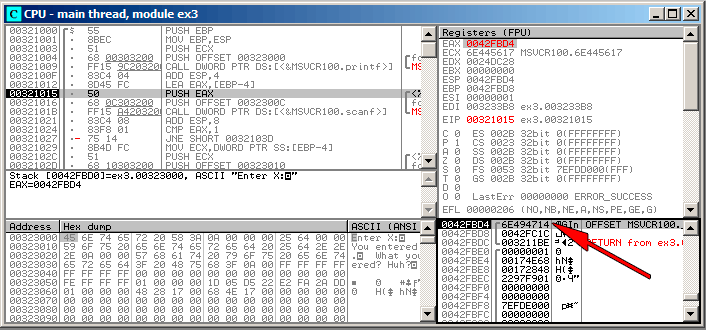
\includegraphics[scale=\FigScale]{patterns/04_scanf/3_checking_retval/olly_1.png}
\caption{\olly: passing variable address into \scanf}
\label{fig:scanf_ex3_olly_1}
\end{figure}

\clearpage
While \scanf executes, in the console we enter something that is definitely not a number, like \q{asdasd}.
\scanf finishes with 0 in \EAX, which indicates that an error has occurred:

\begin{figure}[H]
\centering
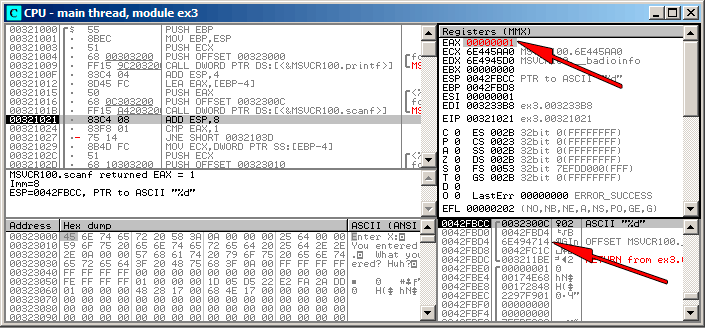
\includegraphics[scale=\FigScale]{patterns/04_scanf/3_checking_retval/olly_2.png}
\caption{\olly: \scanf returning error}
\label{fig:scanf_ex3_olly_2}
\end{figure}

We can also check the local variable in the stack and note that it has not changed.
Indeed, what would \scanf write there?
It simply did nothing except returning zero.

Let's try to \q{hack} our program.
Right-click on \EAX, 
Among the options there is \q{Set to 1}.
This is what we need.

We now have 1 in \EAX, so the following check is to be executed as intended, 
and \printf will print the value of the variable in the stack.

When we run the program (F9) we can see the following in the console window:

\begin{figure}[H]
\centering
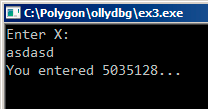
\includegraphics[scale=\FigScale]{patterns/04_scanf/3_checking_retval/olly_3.png}
\caption{console window}
\end{figure}

Indeed, 1850296084 is a decimal representation of the number in the stack (\TT{0x6E494714})!
